\chapter{Results}
\section{Dynamics}
Early versions of the robot used arbitrarily chosen scaling to approximately get the motions right, but a more numerical concert approach based on the dynamics of the system was desired to tune the parameters. The dynamics of the system start at the servo inputting an angle, which then transfers through numerous pin linkages before finally being outputted by the camera seen by the computer. As such, a test was set up to find the relationship between the servo angular displacement and the resulting planar image movement. The test was done by making a custom Python script that only controlled a single axis at a time. The script would record the center of the recognized face, while the user looked at it keeping their face as still as possible, then advance the angle of the servo by 3 degrees, then repeat. This loop ran until the face had moved out of frame of the camera and the software could not see a face anymore. The stepper motor was tested the same way, just was instead told to advance 100 steps every loop. The tests were done over three trials and averaged. The results of the data are plotted in a scatter plot form in Figure \ref{fig:scatter}.

\begin{figure}[h]
    \centering
    \begin{subfigure}{0.475\linewidth}
    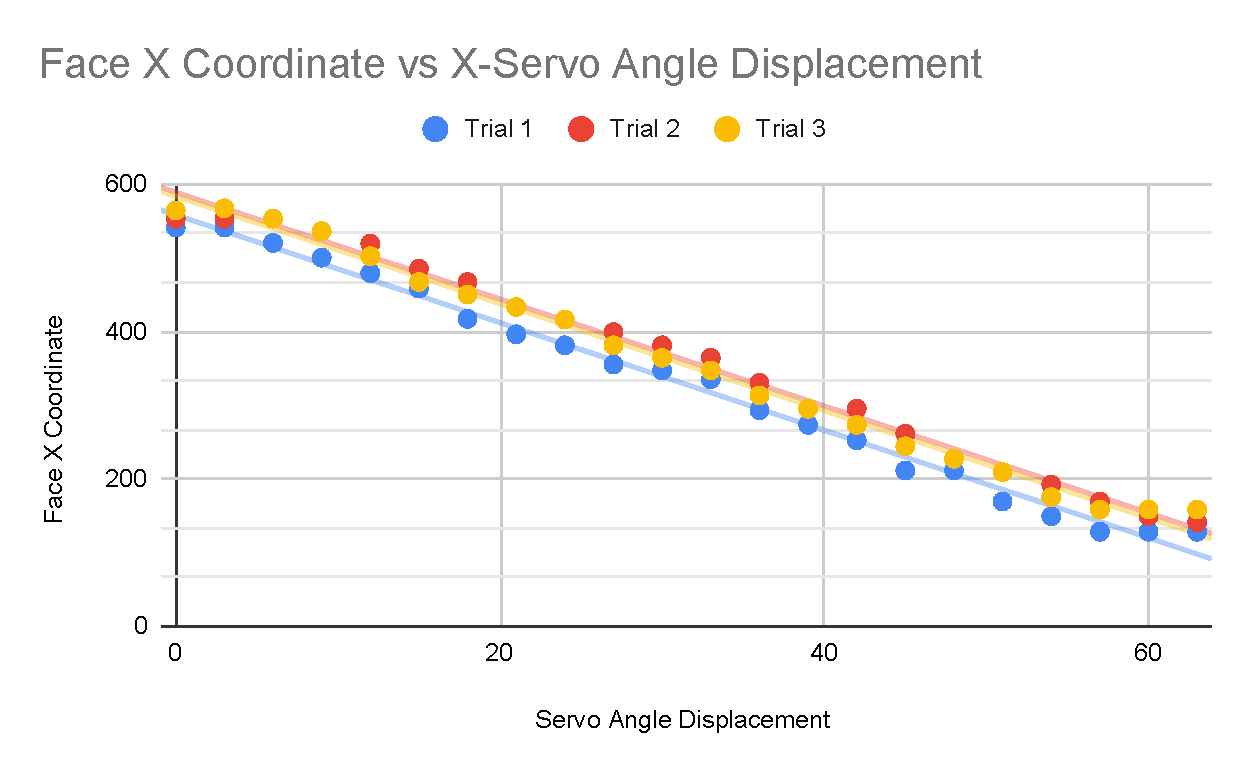
\includegraphics[width=\linewidth]{Thesis/ch5/Face X Coordinate vs X-Servo Angle Displacement.pdf}
    \end{subfigure}
    \begin{subfigure}{0.475\linewidth}
    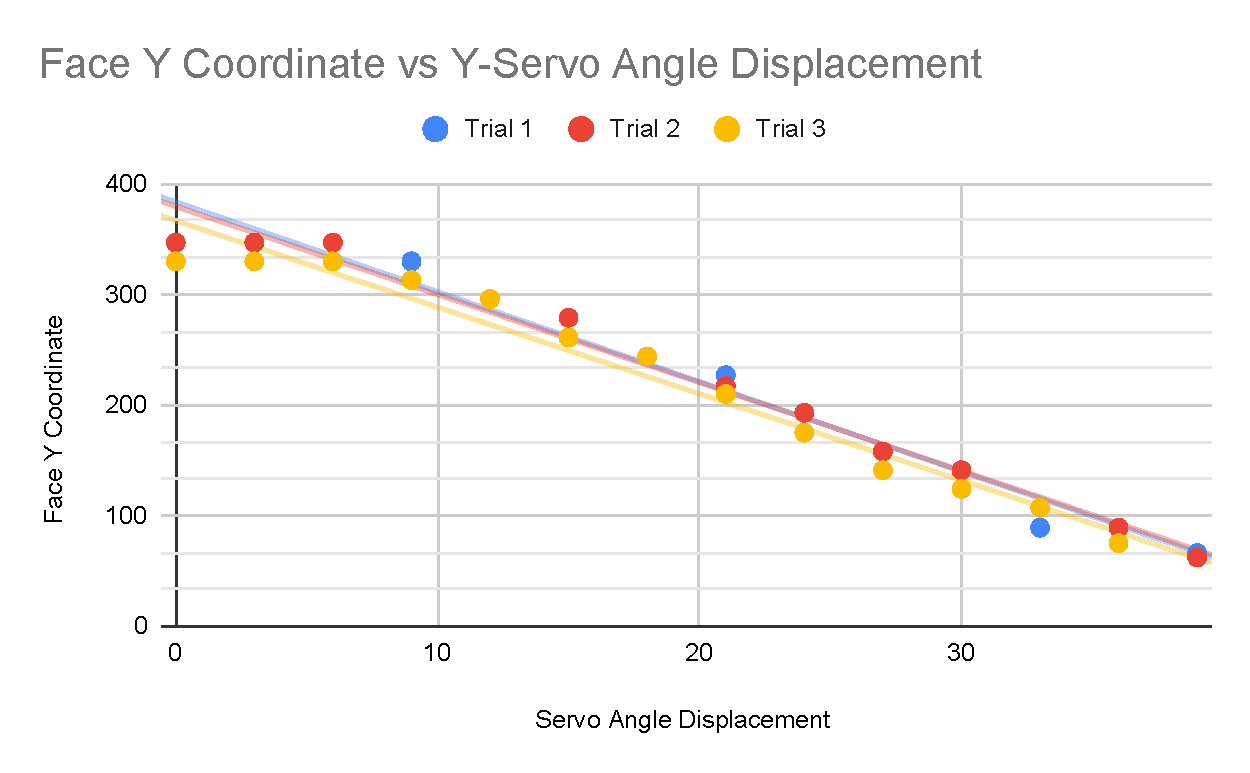
\includegraphics[width=\linewidth]{Thesis/ch5/Face Y Coordinate vs Y-Servo Angle Displacement.pdf}
    \end{subfigure}
    \begin{subfigure}{0.475\linewidth}
    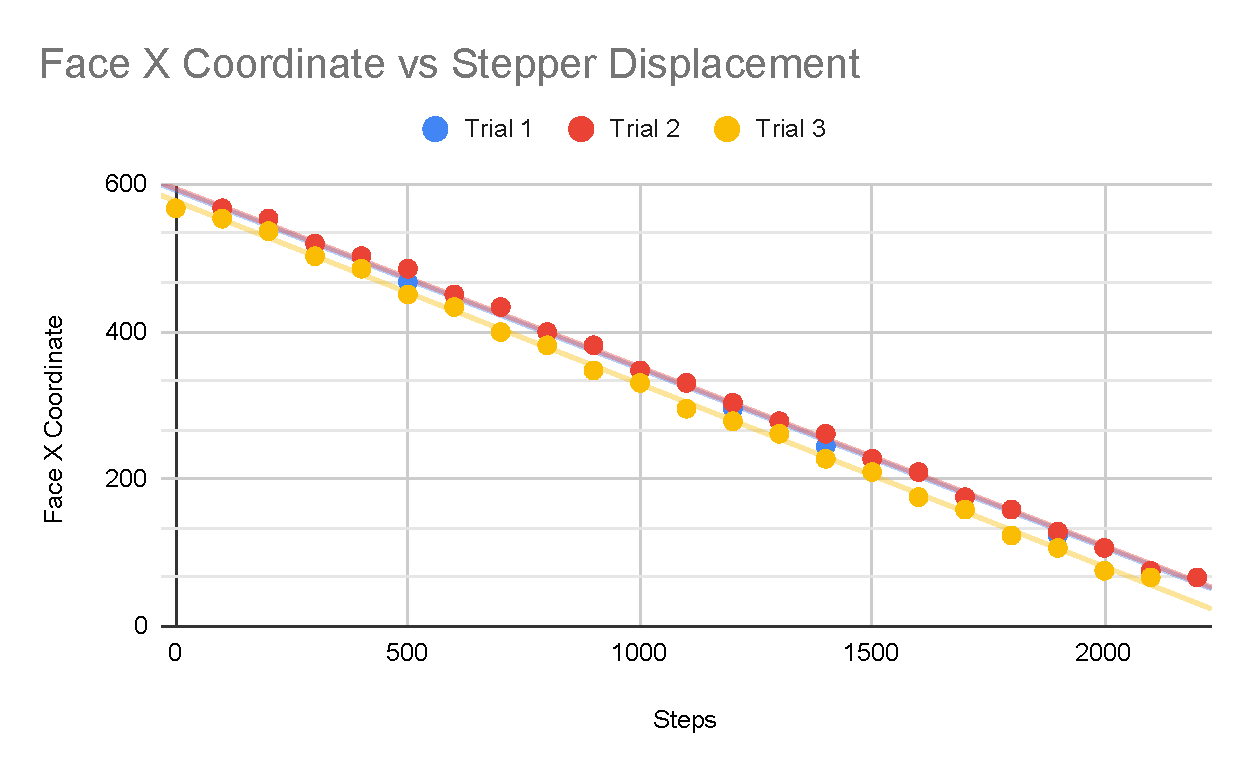
\includegraphics[width=\linewidth]{Thesis/ch5/Face X Coordinate vs Stepper Displacement.pdf}
    \end{subfigure}
    \caption{Scatter Plots of Resulting Face Location}
    \label{fig:scatter}
\end{figure}

A line of best fit was calculated using the data collected in the tests. The slope of the line of best fit was found for each trial and then averaged for a final result, shown in Table \ref{tbl:averages}. It was found that for the Y-Servo, for every degree the servo arm moves, the face in the image moves by 7.98 pixels. The results for the X-Servo were similar, with a slope of 7.28. For every step of the stepper motor, it was found that the image moves 0.25 of a pixel. This makes sense since a full revolution of the robot would require 19200 steps, so step commands sent to the motor should be much higher than the servo command to move the same angular displacement. The results of these tests were then used to inform the parameter values of the motor commands in the Python script. The values are used as the scaling factor that converts the distances in the image to the servo movement commands, as seen in Appendix \ref{ch:python-code}. 

\begin{table}[h]
    \centering
    \caption{Average slope of regression line for 3 trials.}
    \label{tbl:averages}

    \begin{tabular}{c|c|c|c|c}
         & Trial 1 & Trial 2 & Trial 3 & Average\\
        \hline
        Y-Servo & -8.133 & -7.972 & -7.835 & -7.980\\
        X-Servo & -7.302 & -7.253 & -7.280 & -7.278\\
        Stepper Motor & -0.242 & -0.243 & -0.248 & -0.244\\
    \end{tabular}
\end{table}

\section{Speed and Acceleration}
From the datasheet of the servo, the maximum rotational speed of the servo is 0.16 sec/$60^\circ$, which corresponds to 6.54 rad/s. Early versions of the algorithm drove the motors at their maximum speed, but this produced a jarring and jerky movement. Moreover, rapid movements of the camera cause the image to blur and impede the facial recognition accuray. For this reason, the speed of the servos were limited in the software. As such, the ServoEasing and AccelStepper libraries were used in Arduino to add smooth acceleration and deceleration to the eye movements to make them more natural and inviting. This set a software limit to the speed and acceleration of the robot, The speed was set to 80 degrees/sec in software, which corresponds in the real world to 0.98 rad/s. The X servo was also set to this value, but since the microseconds limits were different this corresponds to 0.75 rad/s. There was no acceleration set for the servos to give them a faster response time. In fact, servo motors have a slight wind up naturally as the motor overcomes its stationary inertia, which another reason why software acceleration was deemed unnecessary.

Similar reasoning applied to the stepper motor. The torque curve of the motor provided by the manufacturer indicates that the maximum speed of the motor is around 4000 half steps per second, which corresponds to a rotational speed of 1005 rad/s. Not only is this much too fast for normal operation, but also the torque of a stepper motor drops off at higher speeds, therefore the max speed was set to 3000 step/s in the software, which corresponds to 15.7 rad/s after the 1:6 gear ratio. The maximum acceleration of the stepper motor set to 1000 steps/s$^2$ to give it an ease-in ease-out animation. This corresponds to a real-world rotational acceleration of 5.24 rad/s$^2$.

\section{Time}
\label{ch:time}
With these parameters set, the actual output of the robot had to be measured to validate its performance. For this purpose, the time required for the robot to cycle through the full field of vision was recorded. The results of this test are shown in Table \ref{full-move-times}. This was done with a custom script that swept the two stepper motors through their full range of motion and another script that did the same for the stepper motor. Since the eye servos are synchronized in the software such that they will always reach their end points at the same time, both servos were timed simultaneously producing a single measurement, as shown in Table \ref{full-move-times}. The average time for the eye mechanism to sweep from one side to the other was 4.248 seconds. The average time for the motor to sweep from $-180^\circ$ to $+180^\circ$ was 5.936 seconds. Ignoring acceleration,this corresponds to an average rotational velocity of 0.26 rad/s for the Y-Servo and 0.20 rad/s for the X-Servo, which is well within the bounds set in the software. The stepper motor is moving at an average velocity of 1.06 rad/s, which also falls within the maximum value set in the software. This ensures the safety of the user as the robot will not behave unpredictably and move faster than the software tells it to, even when it is making movements over the complete range of motion.

\begin{table}[h]
    \centering
    \begin{tabular}{c|c|c}
    Trial & Servos & Stepper \\
    \hline
    1&4.28&5.81 \\
    2&4.57&6.06\\
    3&4.15&6.17\\
    4&4.13&5.75\\
    5&4.11&5.89\\
    \hline
    Average&4.248&5.936
    \end{tabular}
     \caption{Measurements on the amount of time required for the motors go through a full move.}
     \label{full-move-times}
\end{table}


\section{Field of View}
\label{ch:fov}
According to B\&H Photo Video, the camera has a base field of view of 78 degrees \cite{b&hphotovideoLogitechC615Webcam}. The camera output is 16:9 ratio, but unfortunately the Python library crops the image to 4:3 for the facial recognition to work, so a test was done to find the resulting field of view after all the software distortions. The facial recognition software was set to run in a loop. I then moved myself to the very edge of the frame, where if I moved even slightly in one direction my face would stop being registered. Then, a marker was placed on the floor directly below me. This was done three times in both directions for a total of 6 measurements. Then, a line was drawn through these points and insersected at a point. The angle between the two lines is the measured field of view of the camera. The field of view was found to be around 60 degrees, shown in Figure \ref{fig:basic-fov}. 

However, with the actuation of the motors, it can be said that this affords the device a much better effective field of view. Since the eye can rotate the camera left and right, this allows the camera to see more of its environment. As such, a similar test was run with the camera panned to its maximum angle left and right, measurements were taken, and the angle between the lines was measured. With the range of motion the effective field of view was measured to be $130^\circ$. Figure \ref{fig:actuated} shows this in the green portion. The stepper motor also increases this field of vision. Since it can move through a full $360^\circ$ range of motion, this increases the effective field of view of the robot to $360^\circ$. This can be seen in the diagram as the blue circle.

\begin{figure}
    \centering
    \begin{subfigure}{0.4\linewidth}
        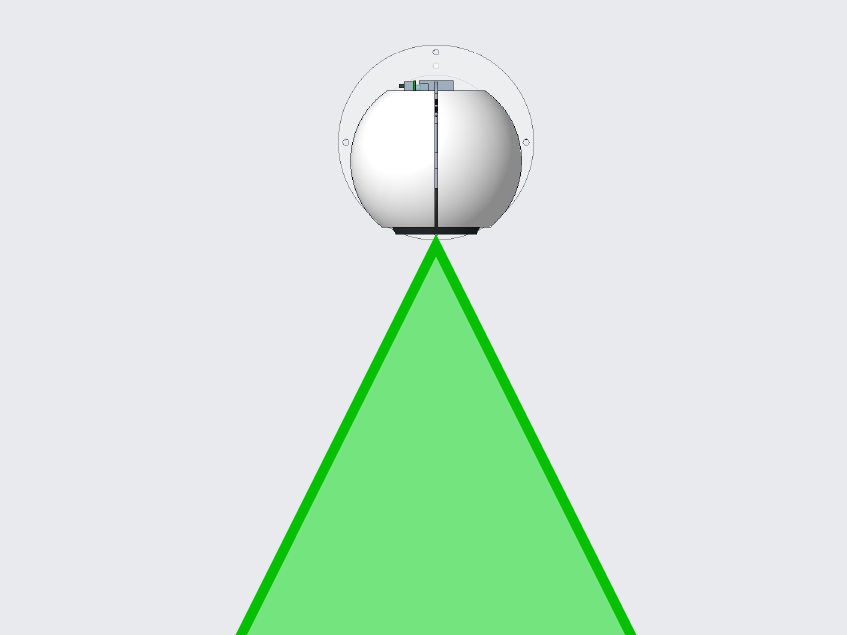
\includegraphics[width=\linewidth]{Thesis/ch5/old-fov.png}
        \caption{}
        \label{fig:basic-fov}
    \end{subfigure}
    \begin{subfigure}{0.4\linewidth}
        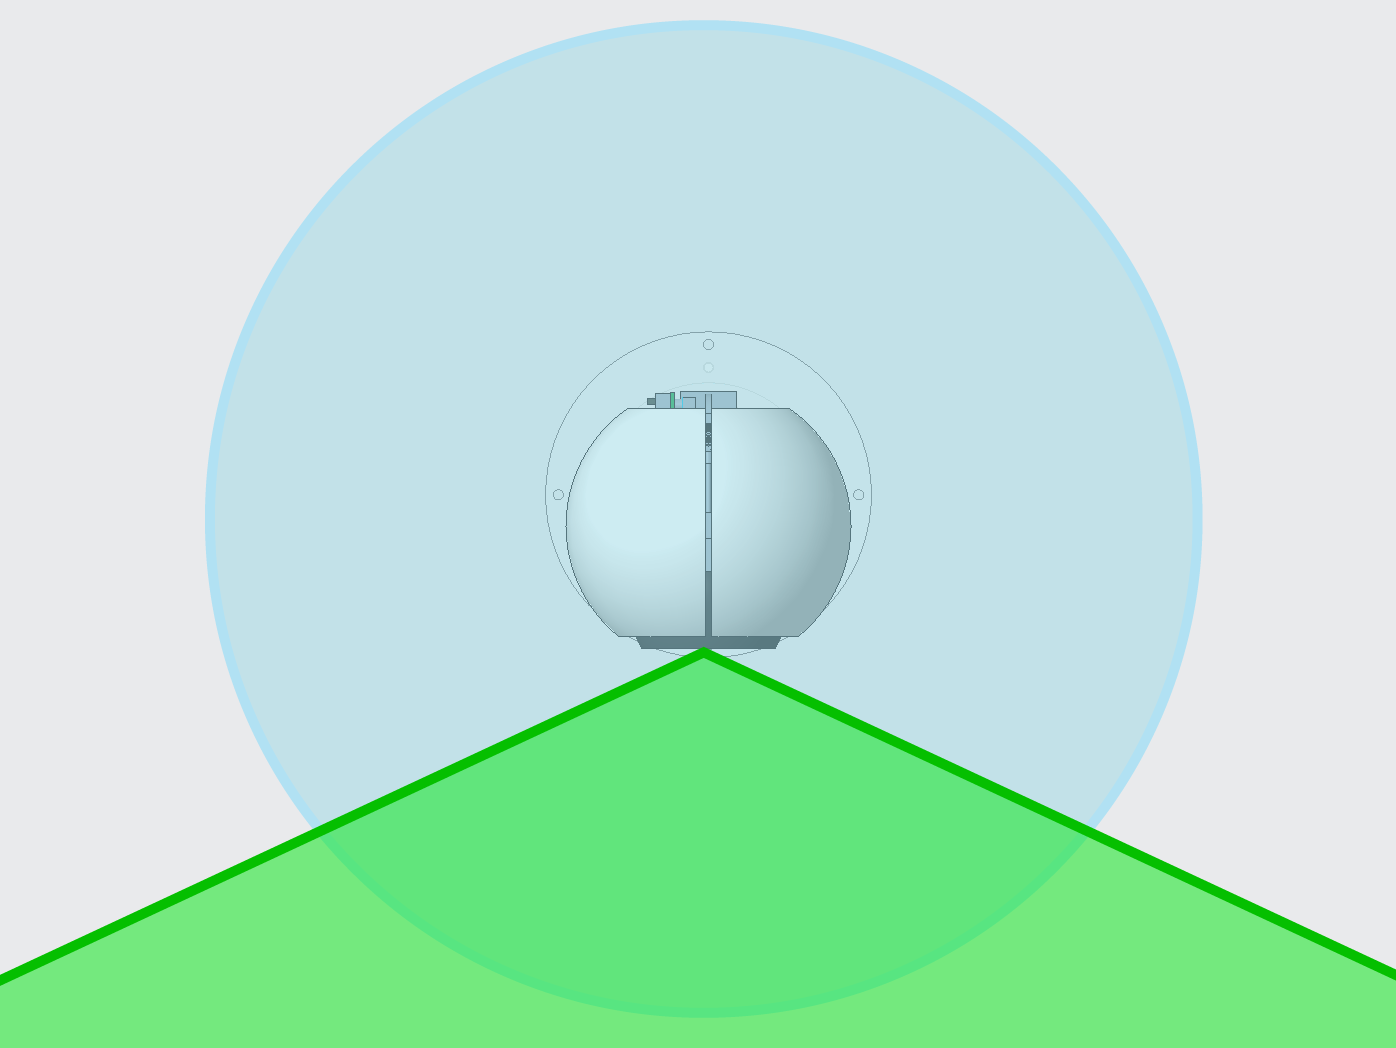
\includegraphics[width=\linewidth]{Thesis/ch5/new-fov.png}
        \caption{}
        \label{fig:actuated}
    \end{subfigure}
    \caption{Comparison of the base FOV and the effective FOV with actuation.}
    \label{fig:fov}
\end{figure}

\section{Maximum User Movement}
There are some limitations on how fast the user can move relative to the robot. The best results are achieved when the user focuses their eyes on the camera and moves slowly around it. The user must not make sudden jerky movements, otherwise the software will not have enough time to catch up to the face. This can be caused by the servos and stepper moving too slowly to track the person. This was tested extensively and it was determined that the speed of the motors was sufficient. The more significant limitation in in the frequency of the software's measurements.

The facial recognition currently runs every 5 frames of video for performance reasons, with 30fps that is 200ms in between measurements. To be continuously tracked by the camera, the user must move slowly enough so that they are not out of frame by the next time the camera takes a measurement. Since the movement on screen is proportional to how far away you are from the camera, results of this calculation will be expressed per meter away from the camera.

For this to happen in normal operation the user would have to be in the center of the camera's field of view in one measurement frame, and out of the field of view in the next measurement frame. Using the field of view of 60 degrees found in Section \ref{ch:fov}, for every meter you move away from the camera, the distance from the center of the image to the right side of the field of view increases by 2.31 meters. Using this and the 30 fps of the camera, the maximum speed a person could move is 11.55 m/s per meter of distance away from the camera. The vertical distance is the same. Of course a user will not be thinking about their exact numerical speed but it gives a good approximation to help the user use the hardware properly.

To mitigate this issue a wide angle lens could be used to cover the blind spots on the sides of the robot. There are lenses that capture a full 360 degree image and then transform it so it looks normal in software. The resulting planar image would then be able to be fed into the facial recognition library.

\section{Loop Closure Time}
A test was done to find the loop closure time of the loop outlined previously in Figure \ref{fig:control_loop}. The test consisted of standing in front of the camera, moving to a random location, and then standing still and waiting for the robot to start moving. A timer was started every time a movement was made, then stopped the timer once the robot had finished moving. This was repeated 10 times to find an average loop closure time, which is shown in Table \ref{loop-closure-time}. The average loop closure time was found to be 3.1 seconds, which was deemed an acceptable result. A possible explanation for this value being relatively high is that sometimes the camera overshoots or undershoots the face in the image, so the robot gets to approximately the right spot, but then has to make small adjustments before getting the face into the deadzone of the image and finally stopping all movement. This is this algorithm has a trade-off between response time and accuracy. The camera can respond quickly to a large movement of the user by moving the servos a large amount, but by doing so the camera is making a rough estimate, lowering the immediate accuracy of the face tracking. Fortunately though, the system eventually converges as the face approaches the center of the image. To an average user, this is not a huge issue, a person usually does not stand perfectly still when speaking, so tracking a moving target is prioritized more than achieving a stationary resting position.

\begin{table}[h]
    \centering
    \begin{tabular}{c|c}
    Trial & Loop Closure Time (s)\\
    \hline
    1&2.29\\
    2&2.27\\
    3&1.96\\
    4&3.51\\
    5&2.48\\
    6&2.86\\
    7&3.58\\
    8&3.48\\
    9&4.03\\
    10&3.58  \\
    \hline
    Average & 3.1
    \end{tabular}
    \caption{Average loop closure time of the robot.}
    \label{loop-closure-time}
\end{table}

\section{Power Consumption}
To measure the power consumption of the robot, two metrics were collected: the peak current and average current. For the peak current, the custom script from Section \ref{ch:time} was reused to drive the motors through their full range of motion repeatedly. A multimeter was connected in series with the 12V power line going into the motherboard. A video was taken and the maximum current value displayed on the multimeter across 30 seconds of operation was recorded. It was found that the peak current of the robot is 0.88A.

The average current was found using a similar method. The current output of the multimeter was recorded every two seconds for a period of 30 seconds. The results can be seen in Figure \ref{fig:current-graph}. The average current from all these measurements was found to be 0.78A. Using this value, a theoretical battery life for the device can be measured. The battery planned for use would be an 8 pack of rechargeable AA batteries, which would supply a total of 12V and 22.4 Ah. Using the average current measurement it is estimated that the battery life would be 28.79 hours. This is well within a reasonable battery life, so the robot can be used on battery power or plugged into the wall.

Note that battery of laptop running the facial recognition algorithm is neglected, as it is running on its own internal battery and has many background programs running that would make this measurement meaningless.

\begin{figure}[h]
    \centering
    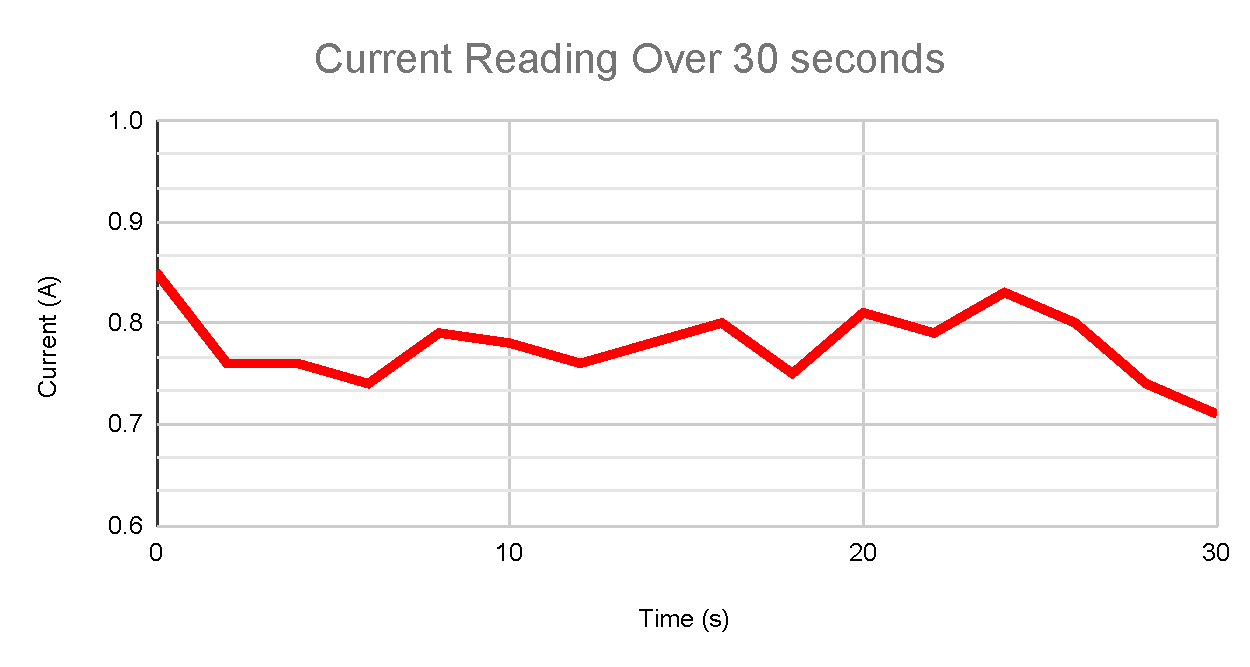
\includegraphics[width=0.7\linewidth]{Thesis/ch5/Current Reading Over 30 seconds.pdf}
    \caption{Current readings taken every 2 seconds for 30 seconds.}
    \label{fig:current-graph}
\end{figure}

\section{Facial Recognition Stress Tests}
The face tracking algorithm currently only supports tracking a single face. The facial recognition library actually outputs an array of possible faces in the image above a default confidence level of 0.6. Since the array is ordered from most confident to least confident, the first element of the array is used in each iteration to calculate the move commands for the motors. An investigation was conducted on how the robot would behave if multiple people were in frame. Figure \ref{fig:two-people} shows the robot's response to this situation. The algorithm simply picks which face it is most confident in and focuses in on it. This purely depends on the dataset used to train the model used in the library, so this is beyond the scope of this project. Also because the confidence is always changing, sometimes the algorithm decides to rapidly switch between faces unpredictably. A topic of future work could explore different ways of making the robot choose which face to focus on and stay focused on. For instance, the robot could focus on whoever is talking. Two microphones could be installed in the robot to discern the approximate lateral position of the person that is speaking. After a certain threshold of noise is reached the camera could point in that direction. This is a possible solution to this problem, but is out of scope for the current iteration of the robot. 

In order for the robot to have consistent operation, the image it receives must be consistent as well. Unfortunately in practice nothing is perfectly consistent, so the algorithm has some issues when running into edge cases. For instance, face tracking performance is diminished in poor lighting conditions. The user has to ensure that their face is fully illuminated and free of obstructions. A test was done to see if wearing sunglasses would be a barrier to the algorithm. An image from this test can be seen in Figure \ref{fig:sunglasses}. It was found that sunglasses interferes with the facial recognition, so the camera opts to focus on another person in the frame. Skin tone was also an issue in the algorithm, as a darker skinned subject was less likely to be focused on.

\begin{figure}
    \centering
    \begin{subfigure}{0.4\linewidth}
        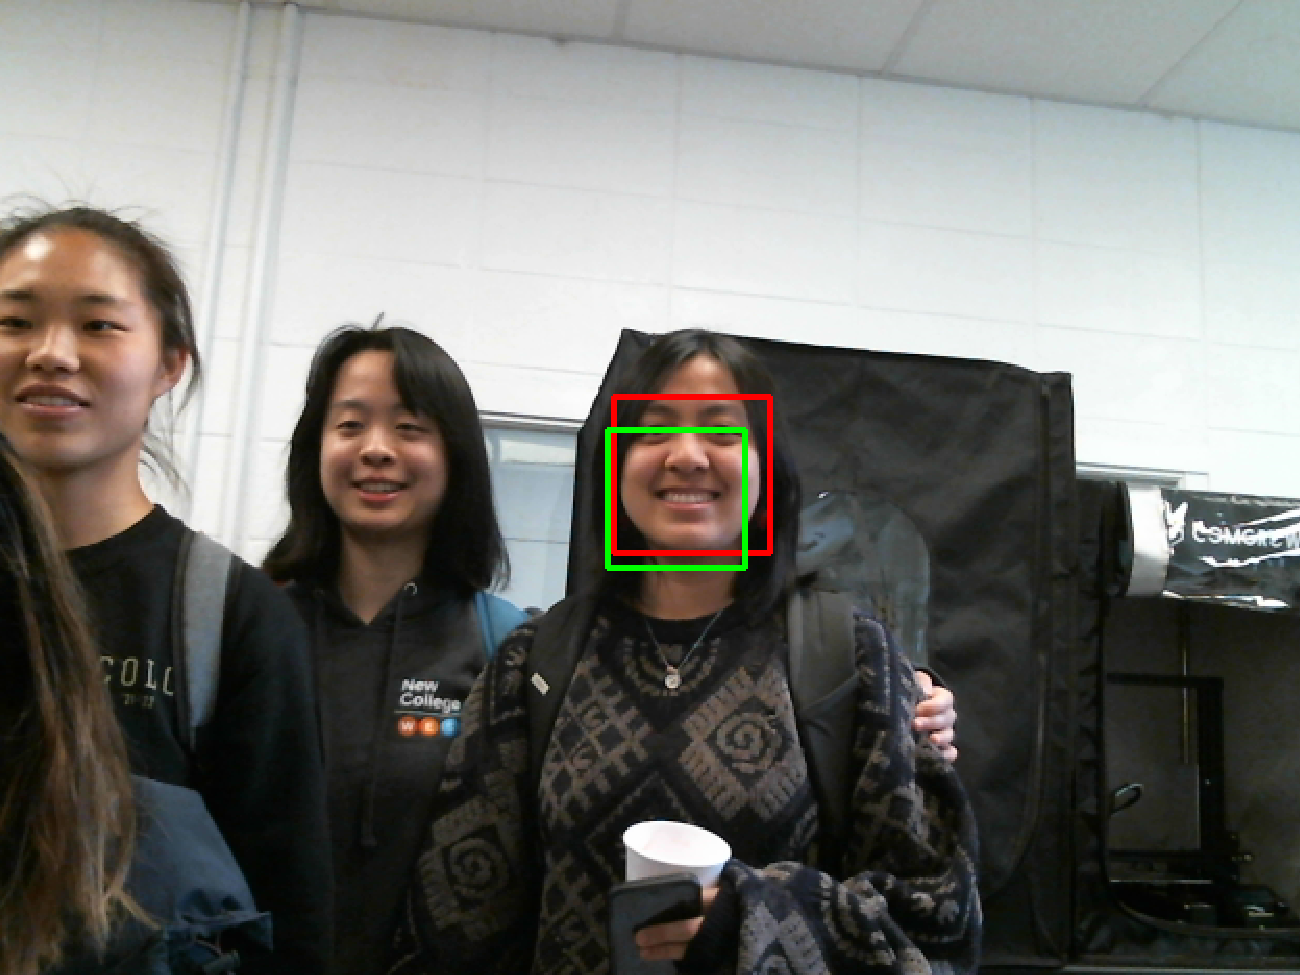
\includegraphics[width=\linewidth]{Thesis/ch5/multiple-faces.png}
        \caption{Multiple people in frame.}
        \label{fig:two-people}
    \end{subfigure}
    \begin{subfigure}{0.4\linewidth}
    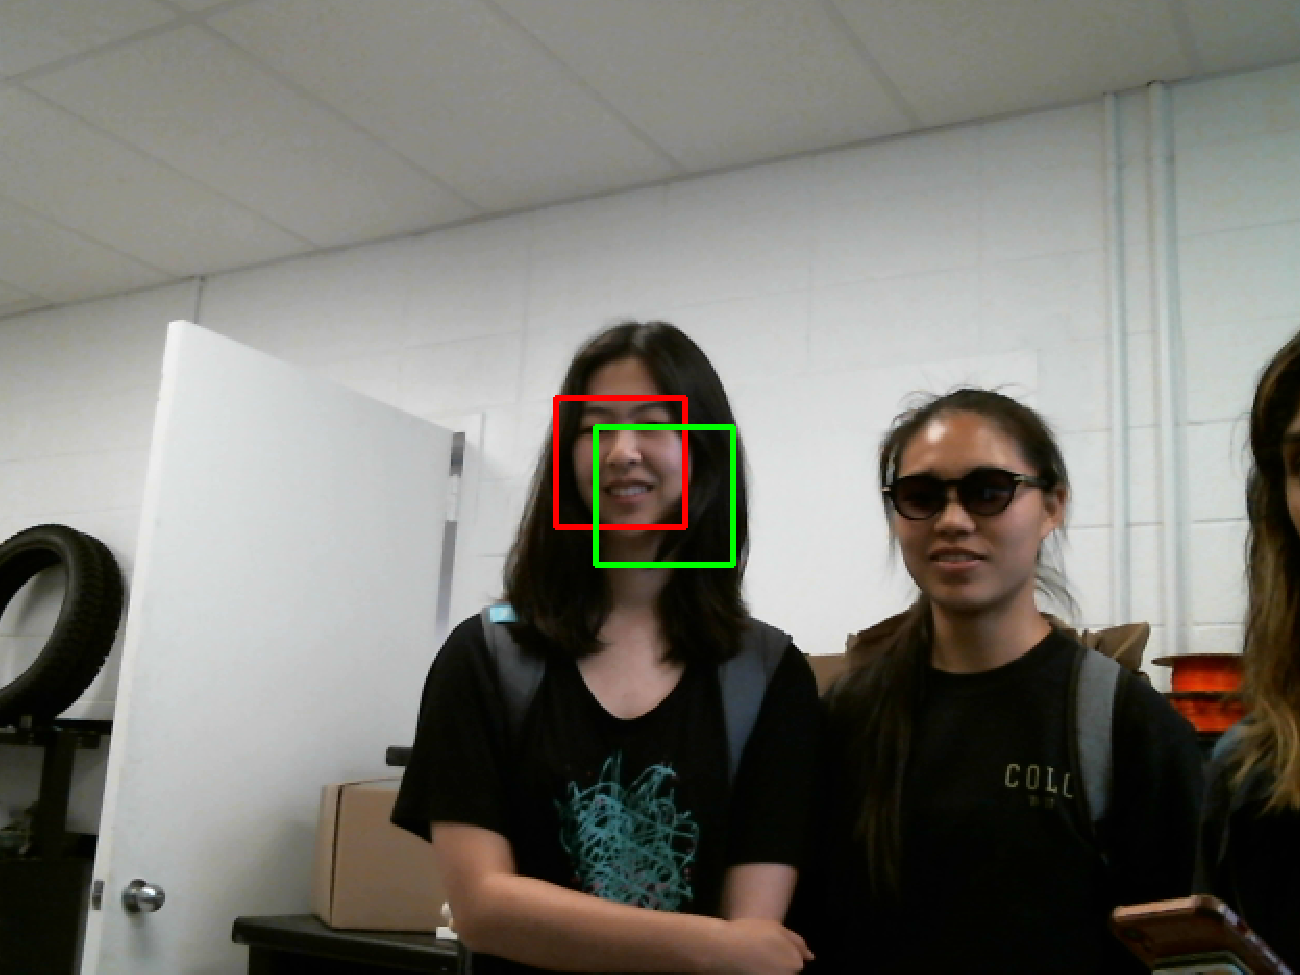
\includegraphics[width=\linewidth]{Thesis/ch5/sunglasses.png}
    \caption{Subject wearing sunglasses.}
    \label{fig:sunglasses}
    \end{subfigure}
    \caption{Examples of challenges to the facial recognition implementation.}
    \label{fig:multiple-faces}
\end{figure}

\section{Peer Feedback}
Informal focus groups were held to gain peer feedback on the robot. After all, the end goal of the project was to make a friendly robot and make people more willing to interact with it. The responses were generally positive. Groups indicated that they would rather speak to this robot than a box like a Google Home, which demonstrates success in that aspect. Negative impressions were given by the people that the robot did not recognize. One participant with darker skin joked that perhaps the robot did not like them, prioritizing another person over themselves. This is unfortunate but ultimately out of this project's control. The main complaint about the robot was the noise. One participant mentioned that if they were in a dark room and heard the growling noise of the stepper motor they would be very frightened. This is a limitation of the components used in this model. Future iterations can add in a more modern stepper driver like the TMC2208 which features silent stepping. People also expected the white part to move with the eye, rather than having the black part be the eyeball and the white part being the head. Perhaps the color scheme of the robot could be another area of future work, where softer colors like brown might be more natural and inviting.